\let\textcircled=\pgftextcircled
\chapter{Literature Review}
\label{chap:related}
This chapter highlights the literature-related work carried out in recent years, along with a discussion of the methodologies adopted in those studies and their identified limitations. Many related works have been conducted using a variety of bioinformatics algorithms, computational tools, and gene expression datasets to explore the genetic and molecular links between diseases, but not for beta-thalassemia and its comorbidities, which is highlighted in this work through a literature review. The main goal of this chapter is to review and discuss the latest literature, methodologies, and findings in this domain, to identify key areas where further research can be undertaken to bridge existing gaps.

\vspace{2mm}
\newpage

\section{Review of Literature}
\label{sec:sec2_1}
Some literature that triggered this study is discussed here:

In \cite{b3} they explored the genetic links between Type 2 diabetes (T2D) and its comorbidities, including kidney failure, liver cancer, myocardial infarction, endometrial cancer, embolic stroke, xanthoma, and xerostomia. They used multiple Gene Expression Omnibus (GEO) microarray datasets for each disease, constructed gene-disease networks (GDNs), performed pathway analysis on KEGG, conducted GO analysis, and built PPI networks. They identified several shared differentially expressed genes (DEGs) between T2D and each comorbidity, suggesting significant molecular associations. However, the study did not include PDI analysis, phylogenetic analysis, or validation analysis, which could have provided stronger clinical insights.

In \cite{b4} evidence suggests that COVID-19 may increase the risk of developing neurodegenerative diseases (NDGDs) like stroke, Alzheimer's disease, epilepsy, Parkinson's disease, and multiple sclerosis. GEO microarray datasets for COVID-19 and these NDGDs were analyzed to uncover shared molecular patterns. The study observed that COVID-19 shared 19, 26, 20, 19, and 22 DEGs with epilepsy, stroke, multiple sclerosis, Alzheimer's disease, and Parkinson's disease, respectively. They mapped disease-gene relationships, explored dysregulated pathways, and built PPI and PDI networks, validating their results.

The study in \cite{b4} also investigates the genetic and pathogenetic similarities between 2019-nCoV (COVID-19) and other coronaviruses, particularly SARS-CoV. They identified hundreds of dysregulated genes using genome alignment, DNA-DNA hybridization, and gene expression comparisons. They constructed an infectome-diseasome network of up- and down-regulated genes, PPI networks, protein-chemical interactions (PCI), and analyzed pathways and gene ontologies. This work aims to understand shared mechanisms between COVID-19 and related viruses for drug repurposing. In contrast, our work focuses on uncovering shared molecular mechanisms between beta-thalassemia and its comorbidities.

The study in \cite{b6} explored the molecular relationships between COVID-19 and its comorbidities, including lung cancer, hypertension, myocardial infarction, and diabetes mellitus. They identified 93 upregulated and 15 downregulated genes in COVID-19, with overlaps of 28 shared genes with diabetes mellitus, 17 with lung cancer, 6 with myocardial infarction, and 7 with hypertension. They performed signaling pathway analysis, GO analysis, PPI and hub protein analysis, PDI analysis, and constructed networks of dysregulated genes. However, this study did not validate their work or perform phylogenetic analysis.

The study in \cite{b7} investigates the genetic connections between gastric cancer and its common comorbidities, including kidney disease, diabetes, stroke, and liver cancer. Using mRNA-seq and microarray datasets, they identified matching shared genes, constructed gene-disease networks, analyzed pathways, ontologies, and protein interactions, and validated their work with benchmark databases. This computational work highlights significant genetic associations between gastric cancer and these comorbid conditions. However, it did not analyze PDI interactions or phylogenetic analysis.

In \cite{b8} the focus was on identifying influential genes (IFGs) in glioblastoma using the Cancer Genome Atlas (TCGA) dataset to understand its genetic links with various comorbidities. They identified 26 dysregulated IFGs from over 16,261 genes through statistical analysis, conducting further analyses including protein-protein and protein-drug interactions, comorbidity networks, and phylogenetic analysis. However, they did not analyze signaling pathways, GO, or validation networks, limiting their work compared to ours.

The work in \cite{b9} identified matching genes among welding fume (WF) and respiratory system diseases (RSDs) by developing a quantitative framework. Using microarray data for WF and RSDs (e.g., asthma, lung cancer, chronic bronchitis, pulmonary edema), they focused on identifying common genes, their networks, pathway analysis, GO analysis, and PPI analysis, validating their results.

The study in \cite{b10} analyzes gene expression to reveal genetic links between Parkinson's disease (PD) and other neurodegenerative diseases (Alzheimer's, ALS, Huntington's, and multiple sclerosis). They identified shared dysregulated genes, pathways, GO analysis, phylogenetic analysis, and protein interactions, validating their findings to highlight PD's potential role in the progression of these disorders.

In \cite{b13} the paper showed bidirectional connections between T2D and breast cancer using GSE 29231, GSE70905, and GSE50586 for diabetes, malignant breast tissue, and both biopsies, respectively. They identified 94 common DEGs, constructed a PPI network, performed limited pathway and ontology analysis, and identified hub proteins and survival construction.

In \cite{b14} differentially expressed genes (DEGs) were identified for colorectal cancer (CRC) and eight related comorbidities. Protein interaction analysis uncovered four sub-networks and eight key hub genes as potential therapeutic targets, predicting clinical outcomes and highlighting genes linked to CRC progression and patient survival. The study reviews machine learning and network-based methods for discovering genetic risk factors for CRC.

The study in \cite{b19} applied bioinformatics and systems biology methods to identify risk factors for cardiovascular disease (CVD) progression. They found 32, 17, 53, 70, and 89 common DEGs between CVD and its associated risk factors, identifying potential biomarkers through PPI analysis, pathway analysis, and ontology analysis, validated using benchmark databases.

\section{Brief Summary of Related Work}
\label{sec:sec2_2}

The existing related works, their methods, datasets, techniques, and limitations are highlighted in Table 2-1 below. The proposed work aims to overcome these limitations after preprocessing microarray and mRNA-seq datasets.

\vspace{5mm} % Remove extra paragraph spacing before table
\begin{longtable}{|p{3.8cm}|p{2.5cm}|p{3.4cm}|p{3.4cm}|}
\caption{Table 2-1 Brief Summary of Related Work} \label{tab:2.1} \\
\hline
\textbf{Authors Name} & \textbf{Datasets} & \textbf{Methods} & \textbf{Limitations of Work} \\
\hline
\endfirsthead
\caption[]{Table 2-1 Brief Summary of Related Work (Continued)} \\
\hline
\textbf{Authors Name} & \textbf{Datasets} & \textbf{Methods} & \textbf{Limitations of Work} \\
\hline
\endhead
\hline
\endfoot
Malik, S.E., Kanwal, S., Javed, J., Hidayat, W., Ghaffar, T. and Aamir, A.H., 2023 \cite{b1} & 135 Beta-Thalassemia Major (BTM) patients & Statistical analysis and laboratory methods & No genetic and molecular relationships \\
\hline
Akiki, N., Hodroj, M.H., Bou-Fakhredin, R., Matli, K., Taher, A.T., 2023 \cite{b2} & Secondary data & Summarizing patterns, mechanisms, diagnostic methods, preventive measures, and treatments reported in the literature & No relationships shown among disease and its comorbidities \\
\hline
Podder, N.K., Rana, H.K., Azam, M.S., Rana, M.S., Akhtar, M.R., Rahman, M.R., Rahman, M.H. and Moni, M.A., 2020 \cite{b3} & GEO microarray datasets & Statistical methods, quantitative model, z-transform, and multi-layered topologies & Fails to calculate large-scale datasets; No drug protein identification; No phylogenetic analysis \\
\hline
Podder, N.K., Shill, P.C., Rana, H.K., Omit, S.B.S., Al Shahriar, M.M.H. and Azam, M.S., 2021 \cite{b4} & mRNA and microarray datasets & Statistical methods and algorithm, and Benjamini-Hochberg algorithm & No phylogenetic analysis; Fails to validate their selected comorbidities \\
\hline
Datta, R., Podder, N.K., Rana, H.K., Islam, M.K.B. and Moni, M.A., 2020 \cite{b7} & Microarray and mRNA-seq datasets & Statistical methods (t-test), z-transformation, multilayer topology, and neighborhood benchmark method & No drug protein identification; No phylogenetic analysis \\
\hline
Podder, N.K. and Shill, P.C., 2022 \cite{b8} & TCGA datasets & Statistical and bioinformatics model & No significant identification of signaling pathway and GO analysis; Fails to validate their work \\
\hline
Rana, M.S., Podder, N.K., Rana, H.K., Hasan, M.I., Azam, M.S., Rahim, M.A., Iqbal, S.H.S. and Saha, S., 2023 \cite{b10} & mRNA and microarray datasets & Benjamini-Hochberg algorithm, neighborhood-based benchmarks, and multilayer topology & Fails to identify protein-drug intersections \\
\hline
Durrani, I.A., Bhatti, A. and John, P., 2023 \cite{b13} & Microarray and mRNA-seq datasets & Integrated in silico analyses approach & No phylogenetic analysis; Fails to identify drug protein \\
\hline
Talihati, Z., Abudurousuli, K., Hailati, S., Han, M., Nuer, M., Khan, N., Maihemuti, N., Simayi, J., Zhang, W. and Zhou, W., 2025 \cite{b14} & TCGA database, genomic database, transcriptomic, and GEO datasets & Limma package in R, STRING database, molecular docking, etc. & Fails to analyze PDI, phylogenetic, and validation analysis \\
\hline
Barua, J.D., Omit, S.B.S., Rana, H.K., Podder, N.K., Chowdhury, U.N. and Rahman, M.H., 2022 \cite{b19} & GEO microarray datasets & Z-transformation, neighborhood-benchmark, and multilayered topology & Fails to identify drug protein; No phylogenetic analysis \\
\hline
Rahman, M.H., et al., 2023 \cite{b25} & GEO datasets & Design matrix model, fit-linear, and Bayesian model & Fails to identify hub and drug proteins; Fails to validate the work; Fails to calculate large-scale data \\
\hline
\end{longtable}

\section{Research Gap}
\label{sec:sec2_3}
Our proposed work offers a more comprehensive level of analysis compared to the referenced studies, as it integrates all analytical approaches previously applied separately in the existing literature. This study comparatively investigates all analyses to explore the deep genetic and molecular correlation of beta-thalassemia with associated endocrine and cardiac diseases. This is shown in Table 2-2.

\vspace{5mm} % Remove extra paragraph spacing before table
\begin{longtable}{|p{1.2cm}|p{2.9cm}|p{3.9cm}|p{2.8cm}|p{2cm}|}
\caption{Comparison of Proposed Work with Related Studies} \label{tab:2.2} \\
\hline
\textbf{Related Work} & \textbf{Datasets} & \textbf{Diseases} & \textbf{DGN, Pathways, GO, PPI, Validation Network} & \textbf{PDI, Phylogenetic Analysis} \\
\hline
\endfirsthead
\caption[]{Comparison of Proposed Work with Related Studies (Continued)} \\
\hline
\textbf{Related Work} & \textbf{Datasets} & \textbf{Diseases} & \textbf{DGN, Pathways, GO, PPI, Validation Network} & \textbf{PDI, Phylogenetic Analysis} \\
\hline
\endhead
\hline
\endfoot
\cite{b3} & Microarray datasets & T2D vs. comorbidities; Gastric cancer vs. comorbidities; Welding fumes vs. respiratory system & YES & NO \\
\hline
\cite{b4},\cite{b6} & mRNA and microarray datasets & COVID-19 vs. comorbidities & YES but Validation: NO & NO but PDI: YES \\
\hline
\cite{b7},\cite{b9} & Microarray datasets & T2D vs. comorbidities; Gastric cancer vs. comorbidities; Welding fumes vs. respiratory system & YES & NO \\
\hline
\cite{b8} & TCGA datasets & Glioblastoma vs. comorbidities & NO but DGN: YES; PPI: YES & YES \\
\hline
\cite{b10} & mRNA and microarray datasets & Parkinson's vs. neurodegenerative & YES & NO but Phylogenetic: YES \\
\hline
Proposed Work & mRNA and microarray datasets & Beta-thalassemia vs. endocrine and cardiac diseases & YES & YES \\
\hline
\end{longtable}

Previous studies on any main diseases and its comorbidities have performed individual analyses such as gene expression profiling, pathway analysis, gene ontology, protein-protein interaction or drug interaction were applied separately and not in an integrated manner. No existing work has combined all of these analytical approaches together to provide a comprehensive genetic, molecular and evolutionary understanding of beta-thalassemia with its associated endocrine and cardiac complications. This gap limits the discovery of common biomarkers, therapeutic targets, and evolutionary insights. Where our work have performed these analyses in combined manner to give a clear and straight visions of BT and its comorbidities connections.

\section{Conclusion}
\label{sec:sec2_4}

This chapter has explored previous research relevant to beta-thalassemia and those research that relevant to system biological approaches. While earlier studies have provided valuable insights into gene expression with its clinical outcomes in a separated manner. But this literature review highlights the absence of an integrated framework that connects genetic profiling with pathway enrichment, ontology, interaction networks and evolutionary perspectives. Recognizing these gaps has guided the direction of the present study, which aims to bring these analyses together to achieve a more clear understanding of beta-thalassemia and its related comorbidities.

% \begin{figure}[H]
% \centering
% % 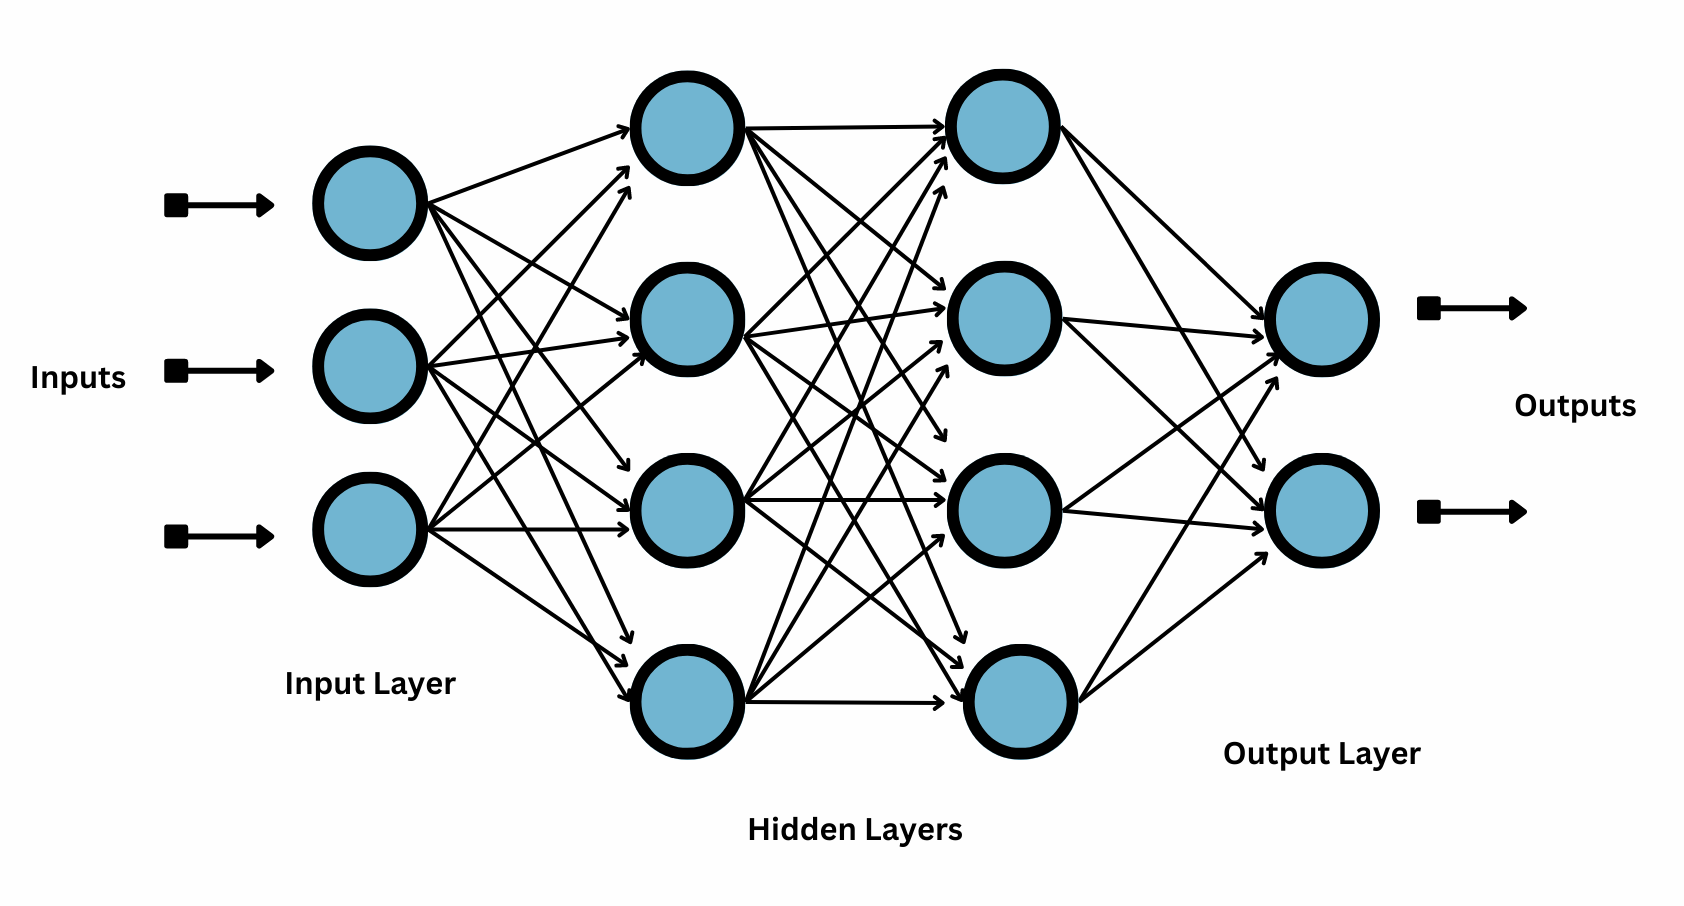
\includegraphics[width=0.9\textwidth]{./images/deeplearncomponents.png}
% \caption{Deep Learning Architecture}
% \label{fig:deeplearn_architecture}
% \end{figure}

